\documentclass[10pt,twocolumn,letterpaper]{article}

\usepackage{iccv}
\usepackage{times}
\usepackage{epsfig}
\usepackage{graphicx}
\usepackage{amsmath}
\usepackage{amssymb}
\usepackage{indentfirst}
\usepackage{subcaption}

% Include other packages here, before hyperref.

% If you comment hyperref and then uncomment it, you should delete
% egpaper.aux before re-running latex.  (Or just hit 'q' on the first latex
% run, let it finish, and you should be clear).
\usepackage[breaklinks=true,bookmarks=false]{hyperref}
\setkeys{Gin}{width=\columnwidth}
\graphicspath{{pictures/}}
\iccvfinalcopy % *** Uncomment this line for the final submission

\def\iccvPaperID{****} % *** Enter the ICCV Paper ID here
\def\httilde{\mbox{\tt\raisebox{-.5ex}{\symbol{126}}}}

% Pages are numbered in submission mode, and unnumbered in camera-ready
%\ificcvfinal\pagestyle{empty}\fi
\setcounter{page}{1}
\begin{document}

%%%%%%%%% TITLE
\title{A Review Of Immersive Scientific Visualization}

\author{Zhongyuan Yu\\
{\tt\small algoyu@163.com}
% For a paper whose authors are all at the same institution,
% omit the following lines up until the closing ``}''.
% Additional authors and addresses can be added with ``\and'',
% just like the second author.
% To save space, use either the email address or home page, not both
\and
Stefanie Krell\\
{\tt\small stefanie.krell@mailbox.tu-dresden.de}
}

\maketitle
%\thispagestyle{empty}


%%%%%%%%% BODY TEXT
\section{Introduction}
%The use of stereoscopic images can improve the depth cue and the perception of the spatial relationships which might be crucial for scientist when analyzing data.
Scientific Visualization is the visualization of scientific phenomena. The purpose is to enable scientists to understand, illustrate and get insight from their data. The data arising from observations or simulations has an implicit or explicit geometric structure, is often very large and most of the time in 3D. Phenomena that can be visualized include the visualization of particles, terrain, volume, flow and tensors.

\setlength{\parindent}{1pc}Virtual reality (VR) can give a sense of presence or immersion in 3D environments. It is a class of computer-controlled multisensory communication technologies that allow more intuitive interactions with data and involve human senses in new ways. An illusion of a three-dimensional world is generated with a stereoscopic head-tracked display system. Nowadays head mounted displays (HMDs) like Oculus Rift1 or HTC Vive2 are widely available and therefore also used in scientific visualization. There are also VR systems like the CAVE (released in 1992) \cite{cruz1992cave}: an immersive virtual reality environment where projectors are directed to the walls of a room-sized cube. It uses a motion capture system, which records the real time position of the user for interaction. VR-systems provide many of the depth cues which we use in the real world, such as binocular disparity and head-motion-parallax. The perception of spatial relationships is highly improved in comparison to 2D displays. When using VR for Scientific visualization, scientists can explore the data in ways which might lead to insights they would otherwise not get because of the increased depth perception and improved interaction with the studied object/phenomena. 

\setlength{\parindent}{1pc}Earliest publications about VR in scientific visualization can be found in the 1990s. Steve Bryson \cite{bryson1994virtual} discussed the use of VR in Scientific Visualization in 1994. He basically concluded that virtual environments provide significant advantages for complex three-dimensional phenomena but drawbacks were high cost of hardware. As technologies evolved costs decrease and display resolutions are higher, VR technologies provide better immersion into a virtual worlds than back in the 90s. Since there has been done a lot of research on this topic in the past decades, we will focus on four new projects from the last 6 years, which are more relevant for today's research. Those projects are using different forms of visualizations: particle visualization, point-cloud visualization and volume visualization. Three of them are using HMDs and one is for the CAVE2 \cite{febretti2013cave2}. We will discuss the rendering techniques and interaction techniques each approach is using. One thing all four approaches have in common is the fact that they have to deal with high amount of data and therefore apply different optimization strategies.

\setlength{\parindent}{1pc}The paper can be divided into 6 chapters. In the second chapter we will present challenges proposed in a approach of point cloud visualization \cite{discher_point-based_2018}. In the following chapter we will discuss a project, which is about tracing neurons in microscopy data \cite{} by. Chapter 4 will discuss a ray-tracing approach for molecular visualization \cite{}. Chapter 5 will describe the techniques used for the visualization of atomistic simulations \cite{reda_visualizing_2013}. The last part will conclude the topic, point out remaining challenges and state some future work.

\section{Point Cloud Visualization}
\subsection{Overview}
Discher et al. \cite{discher_point-based_2018} utilized a multi-pass rendering pipeline to visualize 3D point clouds with different rendering techniques on VR Head Mounted Displays. 3D point clouds are data sets which come from 3D scans e.g. via Airborne (Fig. \ref{fig:pointcloud_1}), Terrestrial or Mobile Laser scanning. They are used in areas like geospatial and non-geospatial applications, building information modeling, urban planning and cultural heritage. Real time rendering of 3D points clouds allows for interactive exploring of real-world assets, sites or regions. As this field has to deal with high amount of data the main challenge is to balance between render quality and performance. In VR on HMDs, the applications have to cope with additional problems: stereoscopic rendering, very high frame rates (90fps as opposed to 30-60fps to avoid nausea, the feeling of motion sickness) and high sensitivity to any kind of visual artifacts which are typical for showing 3D Point Clouds (e.g holey surfaces and visual clutter). The project allows for exploration of 3D point clouds with VR devices such as HTC Vive or Oculus Rift. The algorithm was tested with up to 2.6 billion points. The goal of this project was to show the scalability and practicability of the approach. 

This project is similar to the approaches that are explained in section 3 and 4 as it is designed for visualization on HMDs rather than an immersive environment like introduced in the approach in section 5. Discher et al. \cite{discher_point-based_2018} took a lot of emphasis on the analyzing the visual quality rather than mostly the run time. The visualized data set differs a lot from all the other data sets, because points rather than particles or volumes are visualized.
\begin{figure}
	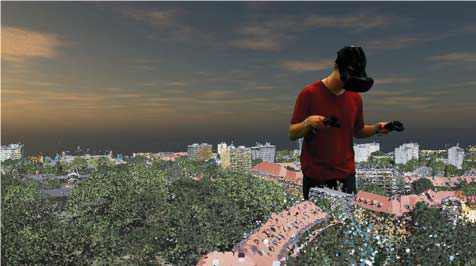
\includegraphics{pointcloud_1.png}
	\caption{Point-cloud Visualization on HTC Vive of an Airborne scan of a city}
	\label{fig:pointcloud_1}
\end{figure}
\subsection{Rendering}
\begin{figure}
		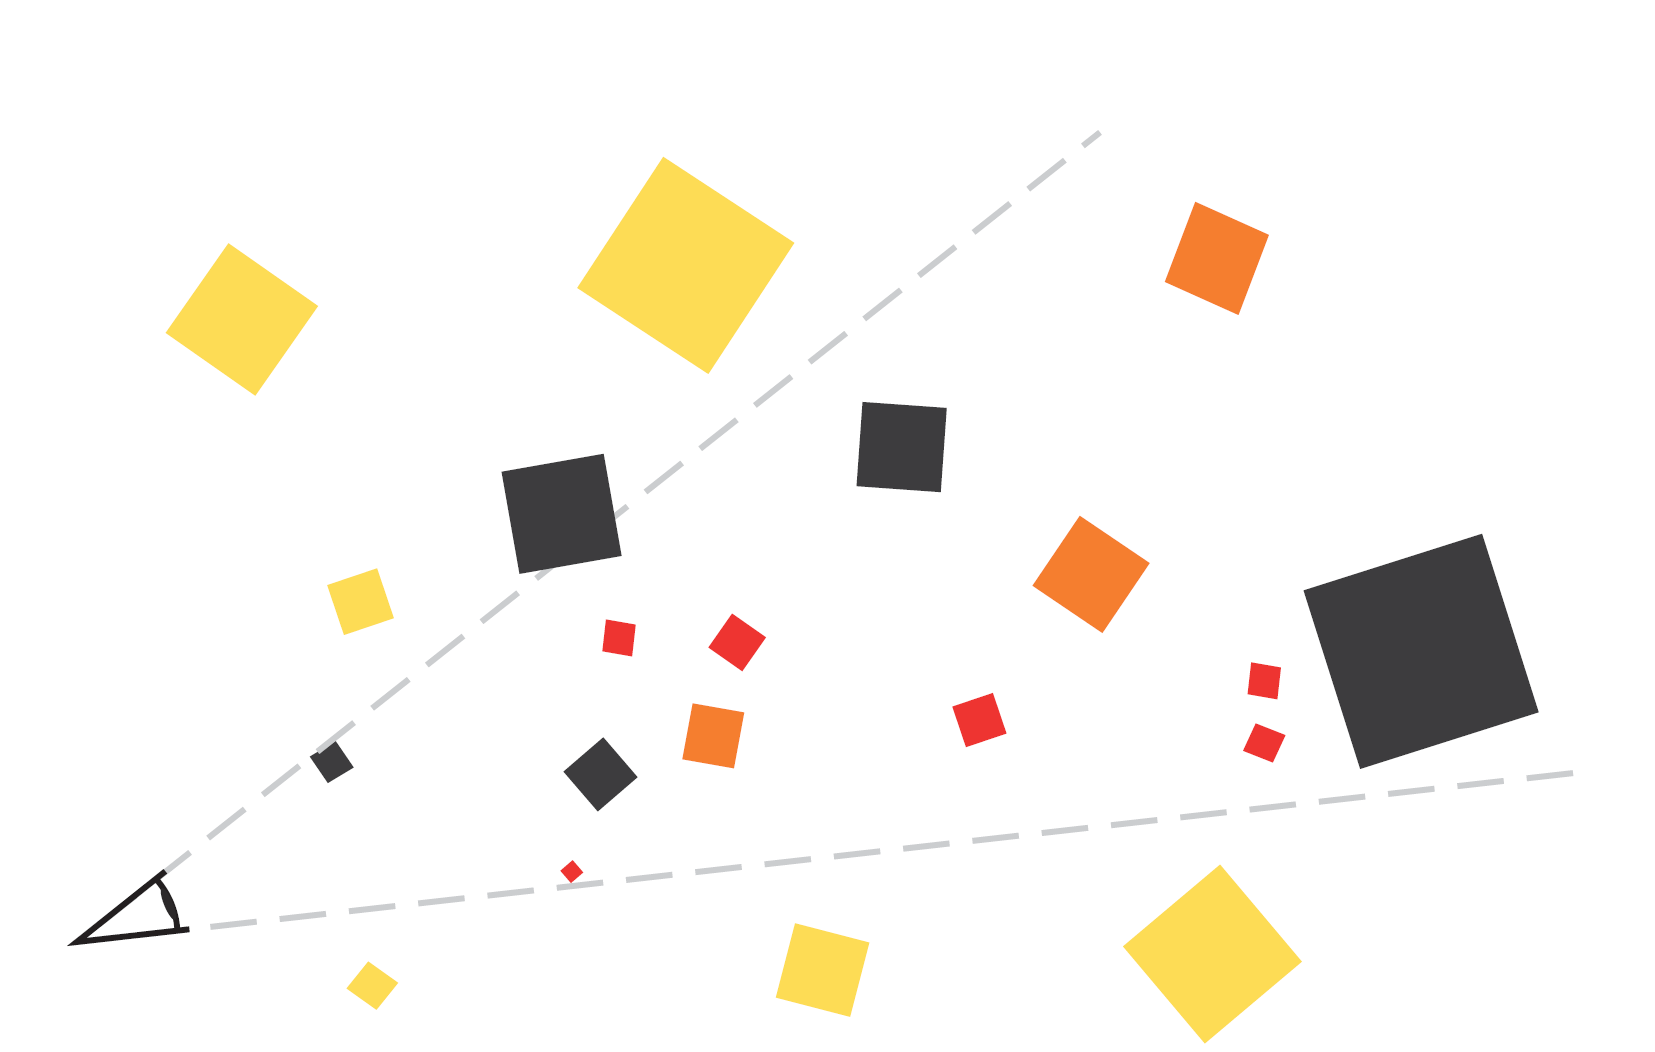
\includegraphics{pointcloud_2.png}
	\caption{Culling techniques used to reduce the amount
of points to be rendered: View frustum culling (yellow),
occlusion culling (orange), detail culling (red).}
	\label{fig:pointcloud_2}
\end{figure}
\begin{figure}
		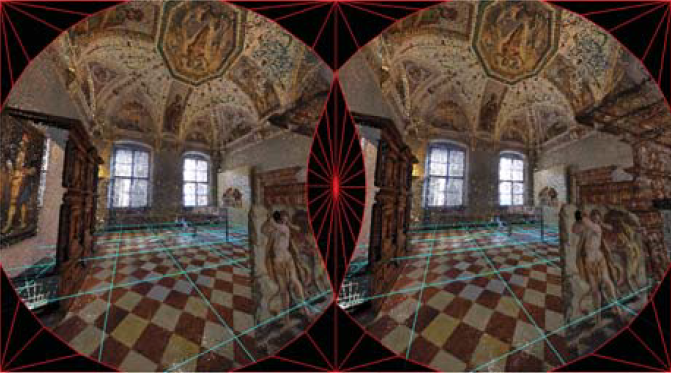
\includegraphics{pointcloud_3.png}
	\caption{A separately rendered mesh serves as a mask to discard fragments beyond the visible area of an VR device’s screens early on}
	\label{fig:pointcloud_3}
\end{figure}
A variety of optimization techniques for rendering were implemented to cope with the performance and visual problems arise when rendering massive 3D point clouds especially on VR devices. Former approaches had to reduce the precision and density of the data by thinning the point clouds \cite{kreylos2008immersive} or converting them into generalized 3D meshes \cite{berger2017survey}. The rendering system of the introduced approach consists of three basic steps: data subset selection, point cloud rendering and image-based post processing.

\setlength{\parindent}{1pc}Data subset selection is necessary because presentation and interactive visualization of 3D point clouds have to deal with the massive amount of data, which generally exceeds available CPU and GPU capabilities. For this reason out-of-core rendering concepts and spatial data structures are required. The 3D point cloud is subdivided in a representative subset that fit into GPU and CPU storage, which can be used for real-time rendering. Here, they determined the subset on a per-frame basis. Firstly, points outside the view frustum are excluded (Fig. \ref{fig:pointcloud_2}). The second technique they used, is detail culling (Fig. \ref{fig:pointcloud_2}). Very small details contribute little. If the estimated area of an object is below a certain pixel threshold, the object is discarded. As an explicit Level-of-Detail (LoD) structure to provide efficient access to the data they are using kd-trees. It is a binary tree whose splitting planes can be chosen on the respective coordinate axes. This allows for minimal traversal times during rendering and the tree structure is balanced independent of the spatial position of points. Other acceleration data structures which have been used for point cloud rendering are quadtrees \cite{Gao:2014:VAL:2619648.2619672} or octrees \cite{kreylos2008immersive}. Schuetz et al. \cite{schuetz-2019-CLOD} proposed a different approach for rendering point clouds in VR. They utilized a continuous LoD structure instead of an explicit one. A flat array is used as a data structure with the hierarchy level stored in an attribute. It exhibits gradual rather than sudden changes in density. The issue which comes due to chunked LoD representation is addressed. It avoids hierarchical traversal, as no tree structure is used. The change of detail is less noticeable. But this approach is limited to point-clouds that fit in GPU memory.

\setlength{\parindent}{1pc}The next step Discher et al. \cite{discher_point-based_2018} called point cloud rendering. The data subset is rendered into g-buffers. That are specialized frame buffer objects (FBO) that combine multiple 2D textures (color, depth, normal). During run time, it is possible to select different rendering techniques and change the appearance of the point cloud. They implemented three different rendering techniques trying to improve the performance. First one is the Hidden mesh rendering (Fig. \ref{fig:pointcloud_3}). The actual visible area on screen on VR devices is restricted to a circular area. To prevent a lot of unnecessary fragment shader operations, a mesh representing the hidden parts of the screen as a mask is used to discard those fragments early on \cite{vlachos_advanced_2015} with early fragment testing. That is possible by using the depth or stencil buffer, which is executed before the fragment shader when using early fragment testing. Next implemented technique is the reverse painters algorithm \cite{foley1996computer}, which is a GPU-based occlusion culling technique based on early fragment testing. Occluded fragments  are not processed by the fragment shader. Scene objects should be rendered in order of their distance to the view position for the technique to have a measurable effect. That is done on a per node basis of the kd-tree rather than per point bases to increase performance. Both of these techniques improved the performance but it varies depending on the number of fragments. The third rendering technique is single-pass stereo rendering, which has the goal to reduce the CPU-overhead by rendering both views of right and left eye in a single render pass \cite{johansson2016efficient}. The frame buffer size is doubled, as each half is assigned to one eye. Instanced rendering, which is a way to render multiple instances of a object in a single draw call and provide each instance with some unique attributes, is used to prevent duplicated draw calls. This technique proved to be less effective because the main performance bottleneck was the GPU rather than the CPU. 

\setlength{\parindent}{1pc}In addition to those, Discher et al. \cite{discher_point-based_2018} implemented two rendering techniques that are supposed to improve the image quality. That is necessary as the impressiveness of a scene is negatively effected by any kind of visual artifact. The most noticeable artifacts due to inappropriately sized points are the holey appearance of surfaces or visual clutter. One technique that was used is the adaptive point size, which works on a per node basis of the kd-tree. For each node they determine its deepest descendant that has been selected for rendering. To all its ancestors the adaptive point size is applied. The point sizes are calculated based on a node’s bounding box rather than its LoD, since nodes of the same LoD might still have quite different point densities. But the visual artifacts are not completely removed. Another rendering technique which was applied is paraboloid rendering \cite{schutz2016potree}. It aims to reduce the visual clutter further by rendering points as paraboloids oriented towards the viewing direction rather than screen aligned disks. A depth offset is added to fragments, which depends on the distance to the corresponding point's center. Undesired occlusions are reduced significantly. But it is not compatible with the rendering techniques using early fragment testing, because the depth is modified in the fragment shader. This technique should only be used carefully as it decreases the performance significantly.

\setlength{\parindent}{1pc}The final step of the used rendering pipeline is imaged-based post processing. It operates on previously generated g-buffers. The post processing should improve the image quality further. Those techniques are screen space ambient occlusion (SSAO) (efficiently approximates the ambient occlusion effect in real-time) \cite{mittring2007finding} and eye-dome lighting (EDL) \cite{boucheny2009interactive}, which add depth cues and highlight silhouettes, blurring \cite{lukin2016tips}, which smooths aliasing and z-fighting (two or more primitives have similar or identical values in the z-buffer). Furthermore, remaining holes are filled and two one-dimensional filter kernels \cite{dobrev2010image} instead of a single two dimensional one for a performance speed up, are applied. The authors of the paper suggested to not use every image improvement techniques as they would slow down the rendering a lot.

\subsection{Interaction}
The VR environment is not only used for displaying. Controllers are used for interaction to improve the experience and exploration. Rotating and scaling of the rendered data is supported, as well as measuring distance between points, and selection of applied rendering technique and color.
\subsection{Conclusion}
The multi-pass approach offers a maximum degree of freedom as rendering techniques can be adjusted at run time. It is highly beneficial for applications in digital documentation, preservation, and presentation of natural and cultural heritage, because it allows user to remotely explore. Future work can focus on performance improvements by distributing the stereo rendering across two separate GPUs.
\section{Tracing Neurons}
\subsection{Overview}
\subsection{Rendering}
\subsection{Interaction}

\section{Molecular Visualization}
\subsection{Overview}
\subsection{Rendering}
\subsection{Interaction}
\section{Visualization of Atomistic Simulations}
\subsection{Overview}
Reda et al. \cite{reda_visualizing_2013} present an application for interactive visualization and exploration of large-scale atomistic simulations in ultra-resolution immersive environments on the CAVE2 \cite{febretti2013cave2} (Fig. \ref{img:atomistic1}). The CAVE2 is a cylindrical immersive environment consisting of 72 micro-polarized, passive stereo LCD panels that are arrange on the circumference of the cylinder, providing a 320-degrees panoramic view at a total stereoscopic resolution of 74 Megapixels. Molecular Dynamics (MD) is a principle methodology in the study of nanoscale systems in applications of alternative fuel, battery design or energy storage. MD simulations usually consist of tens to hundreds of million atoms in complex structures, leading to many challenges in visualization and analysis. Computational chemists, physicists, and materials scientists evaluated the system. Even though there are a lot of molecular visualization techniques, atomistic simulations remain difficult. Real-time rendering of molecular surfaces is also prohibitively expensive. Here they are using a hybrid representation, which combines a ball-and-stick glyph (to show the molecule itself) with volumetric surfaces to show the uncertainty in molecular boundaries at the nanoscale. For evaluation, four different data sets with up to 15 million atoms were used. The goals of the project were to show the scalability and the desire to highlight emergent high-level features in the molecular structure. Furthermore, they wanted to enable scientists to explore different boundary interpretations of atoms or molecules.

\setlength{\parindent}{1pc}This approach has some similarities to the project of chapter 4 as molecules are visualized, but it is difference in the sense that the other project focuses on ray-tracing with the setup of HMDs. Furthermore the project of chapter 3 has some similarities as it visualizing volumetric data as well, but is using isosurface rendering rather than volume rendering.

\subsection{Rendering}
\begin{figure}
	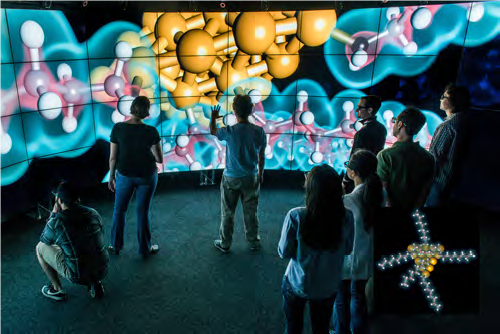
\includegraphics{atomistic_4.png}
	\caption{Visulization of electronic structures}
	\label{img:atomistic1}
\end{figure}
\begin{figure}
	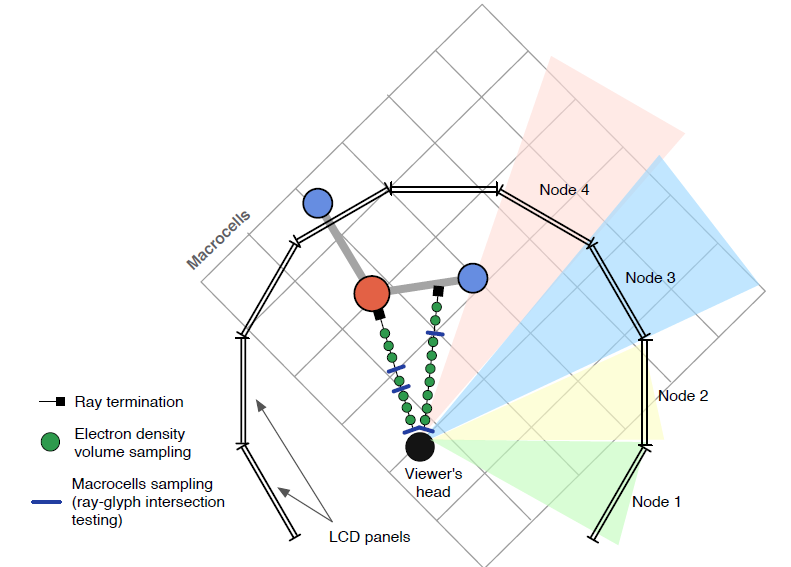
\includegraphics{atomistic_6.png}
	\caption{Illustration of the immersive, distributed ray-casting process}
	\label{img:atomistic2}
\end{figure}
The main techniques they used are ray-casting and volume rendering. Ray-casting is a rendering technique that is done pixel-wise. For every pixel a ray from the viewer is evaluated for intersecting objects. Direct volume rendering is a technique to show a volume data set. Therefore, every sample value is mapped to an opacity and a color via a transfer function. Here, they employed direct volume rendering to render the approximate electron densities. This enables a variety of visual representations by varying the transfer function, which then allows for a flexible interpretation of the molecular boundaries. The volume rendering was very useful for visual classification. For example in one data set (a nanoscale simulation of an amorphous glass (SiO2) fracture), scientists were able to segment the amorphous aluminum shell from the aluminum core. For computational chemists the hybrid volume + glyph technique proved to be more flexible than classical isosurface techniques as they need to see molecule and the electronic structure. The volume rendering also seemed to naturally decrease the visual clutter by creating a 'fog' effect, which reduced the interference with the distant atoms.

\setlength{\parindent}{1pc}As a data structure to represent the ball-and-stick glyphs, a uniform 'Macrocells' 3D grid stored in the GPU is employed. Each voxel in the grid stores information about all of the atoms and bonds, which are within the cell. Therefore only pointers to a separate array are stored, because overlapping glyphs are represented in multiple cells. The ray-casting algorithm \cite{Amanatides87afast} traverses each voxel at a discrete level (Fig. \ref{img:atomistic2}). Because the list of glyphs in a cell is not depth ordered, the algorithm has to test every primitive (sphere or cylinder) against the ray. After a hit is found, the surface of the closest glyph is Phong shaded. Afterward, the charge density volume is sampled within the current cell and the color is accumulated according to the transfer function. Empty Macrocells are skipped and the ray stops when the accumulated volume opacity saturates the pixel- For the electron charge densities, they either used a precomputed electron density grid or a real-time density computation on the GPU. Using precomputed values the algorithm was 2-3 times faster, which was no surprise as the computation is quite expensive. For real time computation of the electron densities they used an approximation with Gaussian distribution based on Van der Waals radii of the atoms or averaged from density functional theory (DFT) computations.

\setlength{\parindent}{1pc}To speed up rendering, an in-core solution was applied making sure that at least one time step of the simulation is loaded into the GPU memory of all rendering nodes. In the CAVE2 \cite{febretti2013cave2} system they employed a 36-node-cluster to render the immersive visualization on 72 LCD panels in parallel. The Ray-cast is done users head to each panel (Fig. \ref{img:atomistic2}). To achieve stereoscopic rendering, rendering and interleaving two images separated by the average inter-pupillary distance is applied. To support correct viewing for multiple individuals, they normalized the head orientation when tracking, so that the eyes are always parallel to the screens surface. That might lead to small distortions between the tiles but it described as a good compromise. 

\setlength{\parindent}{1pc}They were able to achieve real-time interactive rendering when using precomputed electron densities for all of their four tested data sets. Up to 5 million atoms the algorithm scaled solidly with an average frame rate of 15 FPS. With 15 million atoms the frame rate halves but they still achieved interactive rendering at 7 FPS. When the electron densities were computed in real-time, reasonable interactive speeds were achieved for 3 out of 4 data sets. So there are still remaining challenges for optimization of real-time computed electronic densities for atomistic simulations.

\subsection{Interaction}
The CAVE2 \cite{febretti2013cave2} provides 3D navigation using a 6 degrees-of-freedom joystick coupled with head-tracking. The user can fly through the simulation by using a button and by moving/rotating the joystick in the desired direction. Wireless head-tracking also enables the user to explore the visualization by physically walking in the space, causing the view to be rendered from his/her perspective. The head-tracking provides a user-centered perspective. The user can also adjust the transfer function or the color of the electron density ranges by the wireless 'wand' or via separate interface on a tablet or laptop. The modification updates the visualization in real-time. Opacity of the volume and quality of the rendering can also be changed interactively.

\subsection{Conclusion}
As conventional molecular surfaces are not appropriate for many nanomaterials because they do not show the uncertainty in boundaries. The author of the paper showed a hybrid visual metaphor for the visualization complex nanostructured material via volume rendering of approximated electron densities, which proposed advantages. Future work still needs to be done to improve the run-time especially with very large data sets.

\section{Conclusion}

{\small
\bibliographystyle{unsrt}
\bibliography{reviewbib}
}

\end{document}
